\documentclass{article}
\usepackage{graphicx}

\title{Labwork 3: Logistic Regression}
\author{Tran Ngoc Thanh Binh}
\date{May 2026}

\begin{document}

\maketitle

\section{Implementation}

The model uses \textit{Experience} and \textit{Salary} to predict
\textit{Loan}. The linear model is:

\[
z = w_1x_1 + w_2x_2 + b
\]

The prediction is calculated with the sigmoid function:

\[
\hat{y} = \frac{1}{1 + e^{-z}}
\]

The loss function is binary cross entropy:

\[
J = -y\log(\hat{y}) - (1-y)\log(1-\hat{y})
\]

During gradient descent, the error is:

\[
error = \hat{y} - y
\]

The program updates \(w_1\), \(w_2\), and \(b\) for 10000 epochs using a
learning rate of 0.0001. It also plots the decision boundary:

\[
w_1x_1 + w_2x_2 + b = 0
\]

\begin{figure}[h]
    \centering
    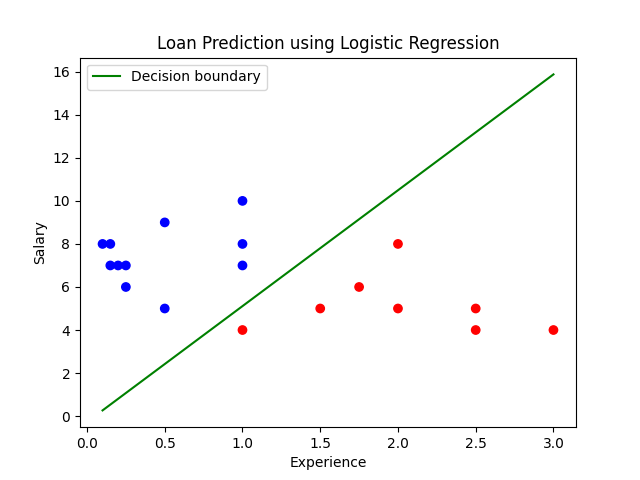
\includegraphics[width=0.8\textwidth]{./Figure_1.png}
    \caption{Loan prediction result with logistic regression decision boundary.}
\end{figure}

\section{Conclusion}

Logistic regression can classify loan results by converting a linear output
into a probability with sigmoid. Binary cross entropy and gradient descent are
used to train the weights and bias.

\end{document}
